%!TEX root = ../main.tex

\chapter{Scheduling problems}
\label{chp:scheduling_problems}

Before starting to tackle the problems that the high propagation delay causes to the \ac{HARQ} protocol, attention shall be put on the random access procedure and on the scheduler, both happening at a lower level, therefore necessary to be able to receive packets.

If those layers are not in working conditions, the communication will not be able to take place.

\section{5G scheduler}
As the name suggests, the main task of the scheduler is to allocate resources to the various connected users in the form of transmission and reception opportunities. In mobile communication networks, the scheduling is dictated by the network and the \ac{UE} has to follow the provided indications.

\subsubsection{5G channels}
The \ac{NR} standard comprises the usage of several channels depending on the type of data to be sent. The medium access control layer is a sort of intermediary, using channels provided by the underlying physical layer and providing the so-called logical channels to the upper layers.

A brief overview of such channels can be found in Table \ref{tab:nr_channels_phy}, listing the ones provided by the physical layer, and in Table \ref{tab:nr_channels_mac}, listing the ones provided by the \ac{MAC} layer. Figure \ref{fig:nr-types-channels} provides a visual clue at the separation in place between the channels at different levels of the protocol stack.

\begin{table}[ht]
    \centering
    \begin{tabular}{|l|l|l|}
    \hline
    \textbf{Transport channel} & \textbf{Acronym} \\ \hline
    Broadcast channel             & BCH         \\ \hline
    Downlink shared channel       & DL-SCH      \\ \hline
    Paging channel                & PCH         \\ \hline
    Uplink shared channel         & UL-SCH      \\ \hline
    Random access channel         & RACH        \\ \hline
    Sidelink broadcast channel    & SL-BCH      \\ \hline
    Sidelink shared channel       & SL-SCH      \\ \hline
    \end{tabular}
    \caption{Transport channels provided by the physical layer \label{tab:nr_channels_phy}}
\end{table}

\begin{table}[ht]
    \centering
    \begin{tabular}{|l|l|l|}
    \hline
    \textbf{Logical channel} & \textbf{Acronym} & \textbf{Type} \\ \hline
    Broadcast control channel             & BCCH     & control     \\ \hline
    Paging control channel                & PCCH     & control     \\ \hline
    Common control channel                & CCCH     & control     \\ \hline
    Dedicated control channel             & DCCH     & control     \\ \hline
    Dedicated traffic channel             & DTCH     & traffic     \\ \hline
    Sidelink broadcast control channel    & SBCCH    & control     \\ \hline
    Sidelink control channel              & SCCH     & control     \\ \hline
    Sidelink traffic channel              & STCH     & traffic     \\ \hline
    \end{tabular}
    \caption{Logical channels provided by the MAC layer \label{tab:nr_channels_mac}}
\end{table}

Different channels are used to convey messages such as the notification of an imminent transmission and the transmission itself, or the uplink scheduling request asked by the \ac{UE} and the successive grant from the base station \cite{5g-mac-devopedia}.

\begin{figure}[ht]
    \centering
    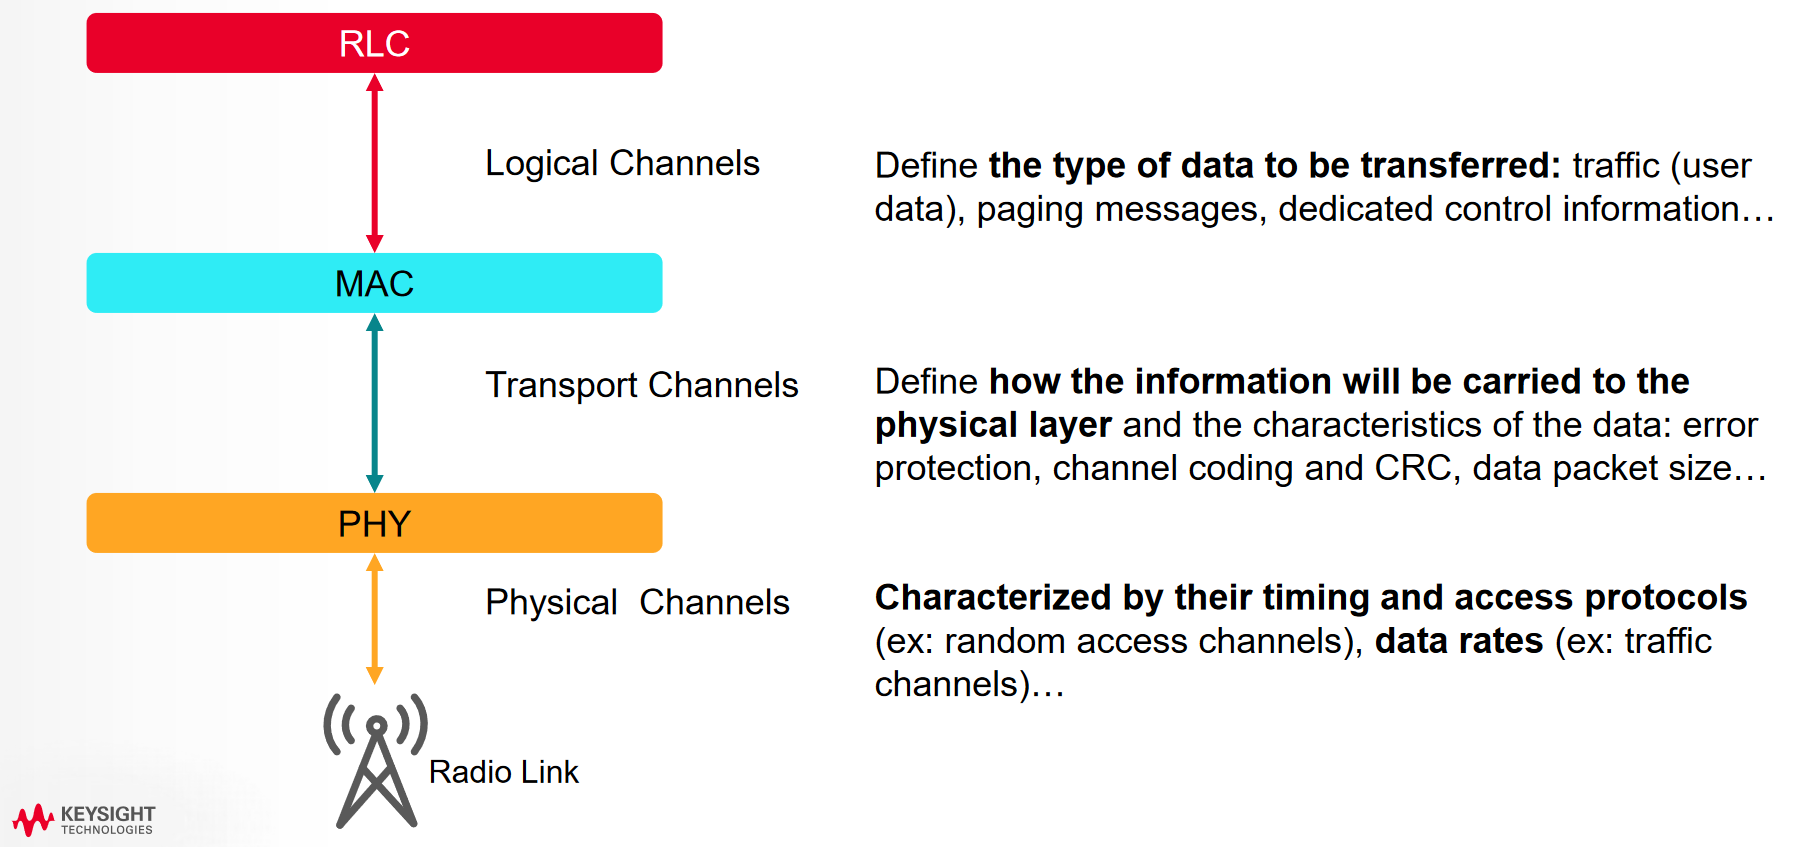
\includegraphics[width=0.9\textwidth]{res/nr-types-channels.png}
    \caption{Different types of channels used in 5G, courtesy of \href{https://www.keysight.com/}{ Keysight technologies}}
    \label{fig:nr-types-channels}
\end{figure}

\subsection{TDD operation}
The most complex problem to solve when dealing with propagation delay is certainly the \ac{TDD} mode of operation. In this scenario, each user can communicate only inside its assigned time slots.

Differently from 4G, where a predefined pattern was in place when allocating downlink and uplink allocations in a radio frame, in New Radio this is done much more flexibly using a plethora of parameters such as the periodicity of UL and DL transmissions, the number of consecutive DL and UL slots and symbols at the beginning of each pattern and more.

\paragraph{}The important key concept is that all the scheduler work has to account for the propagation delay. While in terrestrial communications guard periods of six symbols when switching from downlink communications to uplink communications is sufficient to account for the delay in a 32Km-radius cell, and timing advance commands can account for the different propagation delays experienced by users located in the center of the cell and users located in the cell edge \cite{gsma-5g-tdd-sync}, the same cannot be said for non-terrestrial use cases, where the distances that come into play are much longer, therefore any delay is orders of magnitude higher.

\section{Accounting for propagation delay in scheduling}

\subsection{Problem description}
\label{ss:propdelay-problem-desc}
\paragraph{}
The first encountered problem while implementing a non-terrestrial communication scenario in the simulator was the inability of the scheduler to account for the propagation delay when allocating radio resources to the connected user equipment on the ground.

The implementation of the 5G scheduler in ns-3 is designed to allocate resources less than a single subframe in advance, and since each subframe has a duration time of 1ms, the resource grant was already expired by the time it was able to reach the \ac{UE}, since it was referring to a past subframe.

\paragraph{Example} Consider a scenario with a propagation delay $\tau_p$ of 6ms. The \ac{UE} sends a request for uplink resources at time $t_0$ since it has some data to send. In the terrestrial scheduler implementation, the \ac{gNB} would receive such request at $t_0+\tau_p=6\textit{ms}$ and, provided that other transmissions have not been scheduled yet, grant the \ac{UE} the possibility to transmit in the following slot, which will start after 1ms at $t_0+\tau_p+t_{\textit{slot}}=7\textit{ms}$. However, this grant will reach the \ac{UE} only after another propagation delay, therefore at $t_0+2\tau_p=12\textit{ms}$, when it will already be too late.

\subsection{Proposed solution}
The implemented solution assumes that the scheduler has knowledge of the propagation delay. This is a reasonable assumption since systems such as GPS already rely on a precise estimation of the delay between the user on the ground and the satellite.

The scheduling then proceeds as normal with the only difference being that the information regarding the propagation delay is used to postpone the allocated symbols. 

\paragraph{Example} Consider the same scenario of the previous example in section \ref{ss:propdelay-problem-desc}. The new implementation of the scheduler accounts for the propagation delay by allocating the first available slot after $\tau_p$, so the time for the grant to reach the \ac{UE} is accounted for, and the \ac{gNB} marks the slot after $2\tau_p$ as reserved.

The last part of reserving a different slot is not as immediate. However, this mechanism needs to be in place because of the behavior depicted in Figure \ref{fig:scheduler-allocations-pd}, where a scenario with propagation delay of 5 slots (roughly 1,2ms) is considered:


\begin{itemize}
    \item \ac{UE} sends the scheduling request to \ac{gNB} at frame 1, subframe 0, slot 0.
    \item The \ac{SR} reaches the \ac{gNB} after $1\tau_p$ of 5 slots and the \ac{UE} is scheduled to transmit at frame 1, subframe 2, slot 2 since there is some noticeable propagation delay.
    \item The \ac{SR} reaches the \ac{UE} at frame 1, subframe 2, slot 2, and the \ac{UE} can transmit right away.
    \item The packet reaches the \ac{gNB} after another $\tau_p$, hence the base station needs to know that it cannot schedule other transmissions to take place in this slot, otherwise interference and collisions may arise.
\end{itemize}

\begin{figure}[ht]
    \centering
    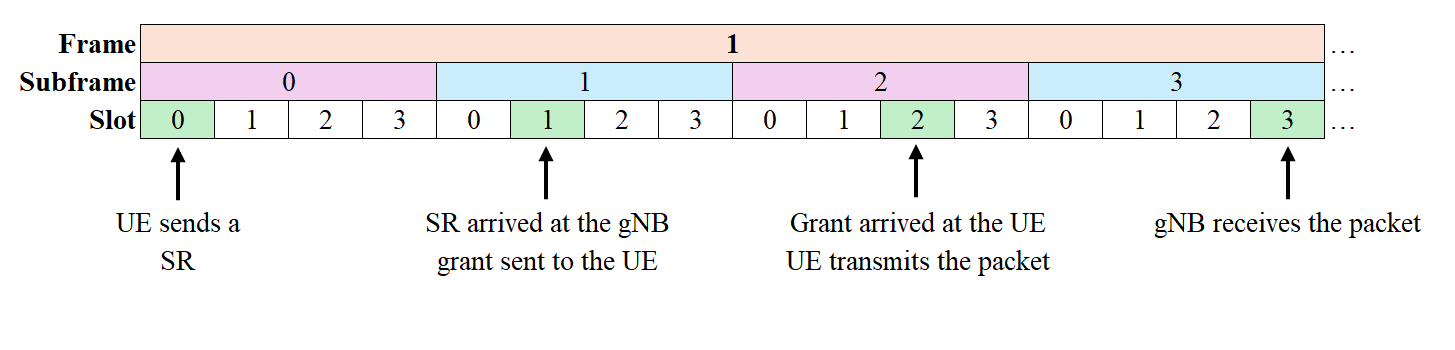
\includegraphics[width=0.9\textwidth]{res/scheduler-allocation-pd.png}
    \caption{Difference between allocated slot and gNB reception}
    \label{fig:scheduler-allocations-pd}
\end{figure}

\section{BSR timer}

After implementing the solution of the previous point in the ns-3 network simulator allowing the communication to take place, some other irregularities were found.
In particular, the 
\todo{Describe how the BSR automatic timeout was discovered, the problem, show the plots in fixed\_distance\_si10\_udp both the physical layer and the e2e throughput, highlighting the difference. Tell how this was fixed increasing the timer. It has to account at least for 2*tp. This is detailed in section 5.4.5 of https://www.etsi.org/deliver/etsi\_ts/138300\_138399/138321/18.01.00\_60/ts\_138321v180100p.pdf}

\section{Inflated BSR}

\todo{Describe the mechanism whenever the send interval was smaller than an RTT, leading to bigger BSR so bigger grants, a lower latency but also some wasted capacity. }

\section{Reordering timer}

\todo{The misalignment between the send interval and the propagation delay leads to the sending of fragmented packets since the grants are always a bit bigger than the packet UE has to send. However, the gNB reordering timer is configured for terrestrial networks, so it expires before we have a chance of receiving the full picture.}